\documentclass[twoside]{article}

\usepackage{epsfig}
\usepackage{amssymb}
\usepackage{amsmath}

\setlength{\oddsidemargin}{0.25 in}
\setlength{\evensidemargin}{-0.25 in}
\setlength{\topmargin}{-0.6 in}
\setlength{\textwidth}{6.5 in}
\setlength{\textheight}{8.5 in}
\setlength{\headsep}{0.75 in}
\setlength{\parindent}{0 in}
\setlength{\parskip}{0.1 in}

\newtheorem{thm}{Theorem}[section]
\newtheorem{Defn}{Definition}[section]

\newcommand{\lecture}[3]{
   \pagestyle{myheadings}
   \thispagestyle{plain}
   \newpage
   \setcounter{page}{1}
   \noindent
   \begin{center}
   \framebox{
      \vbox{\vspace{2mm}
    \hbox to 6.28in { {\bf  ~Probabilistic Graphical Models 10-708 Notes with Koller and Friedman Textbook\hfill} }
       \vspace{6mm}
       \hbox to 6.28in { {\Large \hfill #1  \hfill} }
       \vspace{6mm}
       \hbox to 6.28in { {\it Lecturer: #2 \hfill Scribes: #3} }
      \vspace{2mm}}
   }
   \end{center}
   \markboth{#1}{#1}
   \vspace*{4mm}
}

\begin{document}

\lecture{2 : Directed GMs: Bayesian Networks}{Eric P. Xing}{Xing JunJie} % Lecture name, Lecturer, Scribes

\section{Introduction}

The goal of establishing GMs (Graphical Models) is to represent a joint distribution \(P\) over some set of random variables \(\mathbf{\chi} = \{X_1,\ldots,X_n\}\). Consider the simplest case where each variable is binary-valued, a joint distribution requires total \(2^n - 1\) numbers (minus 1 comes from sum-to-one constraint).This explicit representation of the joint distribution is unmanageable from every perspective\footnote{The following mainly quotes from Koller andFriedman Textbook Ch.3}.

\begin{itemize}
\item \textbf{Computationally}, it's very expensive to manipulate and too large to store in memory.
\item \textbf{Cognitively}, it is impossible to acquire so many numbers from a human expert, and the numbers are very small and do not correspond to events that people can reasonably contemplate.
\item \textbf{Statistically}, if we want to learn the distribution from date, we would need ridiculously large amounts of data to estimate this many parameters robustly.
\end{itemize}

However, \textbf{Bayesian Networks} are able to represent compact representations by exploiting \textbf{Independence Properties}. 

\section{The \emph{student} Example}

We'll introduce perhaps the simplest example to see how \textbf{independence assumptions} produce a very compact representation of a high-dimensional distribution.

We now assume that a company would like to hire some graduates. The company's goal is to hire intelligent employees, but there is no way to test intelligence directly. However, the company have access to student's SAT scores and course grades. Thus, our probability space is induced by three relevant random variables \(I, S\) and \(G\). Assuming that \(G\) takes on three values \(g^1,g^2,g^3\), representing grades \(A, B\) and \(C\), \(I\) takes on two values \(i^0\)(low intelligence), \(i^1\)(high intelligence), \(S\) takes on two values \(s^0\)(low score) and \(s^1\)(high score).

We can get some intuitive independences in this example. The student's intelligence is clearly correlated both with his SAT score and grade. The SAT score and grade are also not independent.If we on the fact that the student received a high score on his SAT, the chances that he gets a high grade in his class are also likely to increase. Thus, we assume that, for our distribution \(P\),\[P(g^1\ |\ s^1) > P(g^1\ |\ s^0)\]

However, it's quite plausible that our distribution \(P\) satisfies a \textbf{conditional independence property}. If we know that the student has high intelligence, a high grade on the SAT no longer gives us information about the student’s performance in the class. That is:
\[P(g\ |\ i^1,s^1) = P(g\ |\ i^1)\]
Generally, we may assume that \[P\models(S\perp{G\ |\ I)}\]

Note that this independence holds only if we assume that student's intelligence is the only reason why his grade and SAT score might be correlated, which means that it assumes that there is no correlations due to other factors. These assumptions are also not ``True'' in any formal sense of word, and they are often only approximations of our true beliefs.
\begin{figure}
\centering
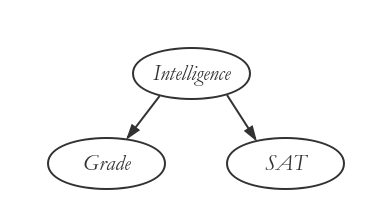
\includegraphics[width=0.3\textwidth]{assets/student_nb.png}
\caption{\label{fig:student_nb}Simple Bayesian networks for the \emph{student} example}
\end{figure}

As in the case of marginal independence, conditional independences allows us to provide a compact specification of the joint distribution. The compact representation is based on a very natural alternative parameterization. By simple probabilistic reasoning, we have that 

\(P(I,S,G) = P(S,G \ |\ I)P(I).\)

But now, the \textbf{conditional independence assumption} implies 

\(P(S,G\ |\ I) = P(S\ |\ I)P(G\ |\ I).\)

Hence, we have that 

\(P(I,S,G) = P(S\ |\ I)P(G\ |\ I)P(I)\)

Thus, we have factorized the joint distribution \(P(I,G,G)\) as a product of three conditional probability distributions (CPDs). This factorization immediately leads us to the desired alternative parameterization. Together with \(P(I), P(S\ |\ I), P(G\ |\ I)\), we can specify the joint distribution. For example, \(P(i^1,s^1,g^2) = P(i^1)P(s^1\ |\ i^1)P(g^2\ |\ i^1)\).

We note that this probabilistic model would be represented using the Bayesian network shown in Figure \ref{fig:student_nb}.

In this case, the alternative parameterization is more compact than the joint. We now have three binomial distributions --- \(P(I)\), \(P(S\ |\ i^1)\) and \(P(S\ |\ i^0)\), and two three-valued multinomial distributions --- \(P(G\ |\ i^1)\) and \(P(G\ |\ i^0)\). Each of the binomials requires one independent parameter, and each three-valued multinomial requires two independent parameters, for a total of \textbf{seven} (\(3 * (2 - 1) + 2 * (3 - 1)\)).By contract, our joint distribution has twelve entries, so that \textbf{eleven} independent parameters.

\section{Bayesian Networks}

Bayesian networks build on the intuition as the naive Bayes model by exploiting conditional independence properties in order to allow a compact and natural representation.However, they are not restricted to the strong independence assumptions naive Bayes model makes.

The core of the Bayesian network representation is a directed acyclic graph (DAG), whose nodes are the random variables in our domain and whose edges correspond, intuitively, to direct influence of one node on another.

We can view  the graph in two ways:
\begin{itemize}
\item a data structure that provides the skeleton for representing \textbf{a joint distribution} compactly in a \emph{factorized} way.
\item a compact representation for \textbf{a set of conditional independence assumptions} about a distribution.
\end{itemize}

\subsection{Factorization Theorem}

Given a DAG, the most general form of the probability distribution that is \textbf{consistent} with the graph factors according to ``\textbf{node given its parents}'':\[P(X) = \prod_{1=1:d}{P(X_i\ |\ X_{\pi_i})}\] where \(X_{\pi_i}\)is the set of parent node of \(x_i\), and \(d\) is the number of nodes.See Figure \ref{fig:factorize_example} for an example.
This graph can be factorized and represented as follows: 
\[
\begin{split}
&P(X_1,X_2,X_3,X_4,X_5,X_6,X_7,X_8) = \\ 
&P(X_1)P(X_2)P(X_3\ |\ X_1)P(X_4\ |\ X_2)P(X_5\ |\ X_2)P(X_6\ |\ X_3, X_4)P(X_7\ |\ X_6)P(X_8\ |\ X_5, X_6)
\end{split}
\]

\begin{figure}
\centering
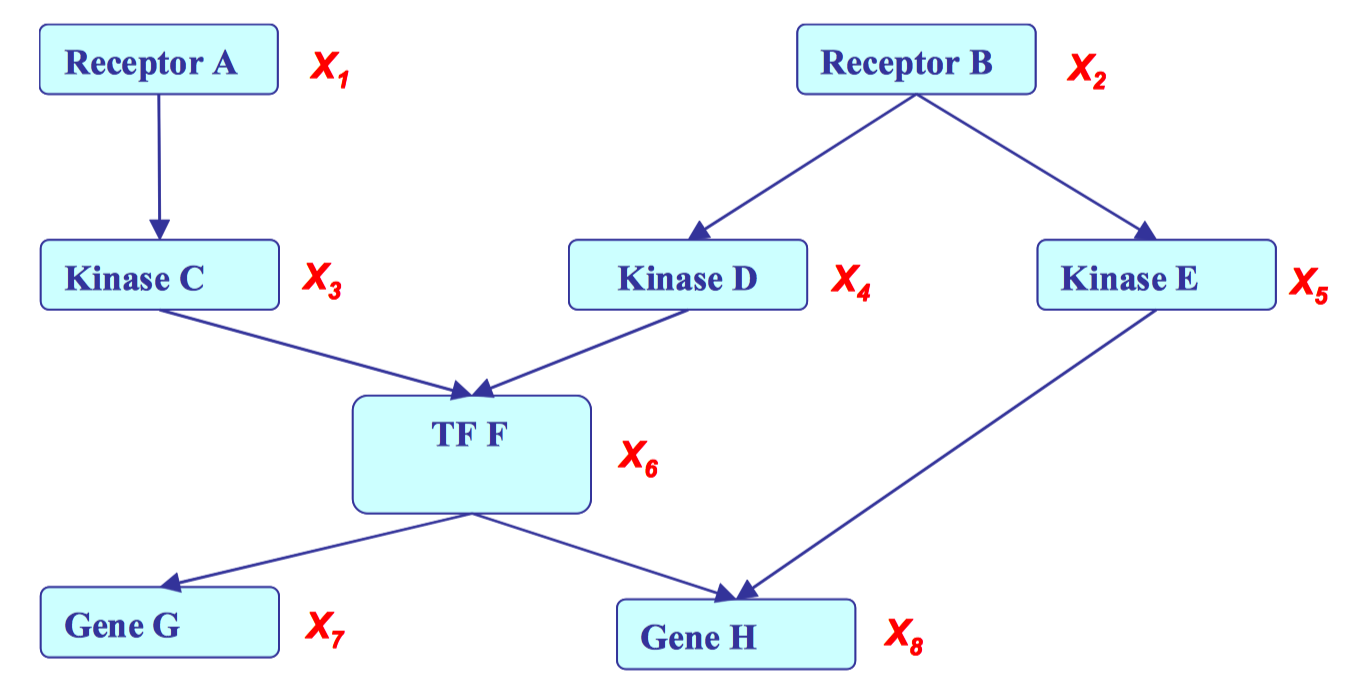
\includegraphics[width=0.6\textwidth]{assets/factorize_example.png}
\caption{\label{fig:factorize_example}Factorize example graph}
\end{figure}

\subsection{Local Structures and Independences}

Graphical models have three fundamental local structures that composes bigger structures.

\begin{itemize}
\item \textbf{Common parent} Fixing \(B\) decouples \(A\) and \(C\). When two variables \(A\) and \(C\) have a common parent \(B\), conditional independence \(A\perp C\ |\ B\) holds.
\item \textbf{Cascade} Knowing \(B\) decouples \(A\) and \(C\). When a middle node in a cascaded three random variables is known, a conditional independence \(A\perp C\ |\ B\) holds.
\item \textbf{V-structure} If \(C\) is not observed, then \(A\) and \(B\) are independent. However, if it is given, then the independence is lost. (\(A\) and \(B\) are not independent given \(C\)). In this case, \(A\) and \(B\) are \emph{marginally independent}.
\end{itemize} 

The unintuitive V-structure can be described by a simple example. Suppose \(A = \) clock on tower, \(B = \) traffic jam on Eric's way to campus, and \(C = \) Eric on time for class. If Eric is not on time and the clock is on time, then our belief that \(B\) occurred is higher.

\section{I-maps}

\begin{Defn}
Let \(P\) be a distribution over \(X\). We define \(I(P)\) to be the set of independence assertions of the form \((X \perp Y\ |\ Z)\) that hold in P.
\end{Defn}
\begin{Defn}
Let \(K\) be an any graph object associated with a set of independences \(I(K)\). Then \(K\) is an \(I-map\) for a set of independences \(I\) if \(I(K) \subseteq I\)
\end{Defn}

For example, if a graph \(K\) is totally connected, then every pair of variables are dependent, more formally, \(I(K) = \emptyset \subset P\). A complete graph is ``useless'', since it does not give any knowledge about the structural.

\subsection{Facts about I-maps}
For \(G\) to be an I-map of \(P\), it is necessary that \(G\) does not mislead us regarding independences in \(P\). In other words, any independence that \(G\) asserts must also hold in \(P\), but conversely, \(P\) may have additional independences that are not reflected in \(G\).

\begin{figure}[!bph]
\centering
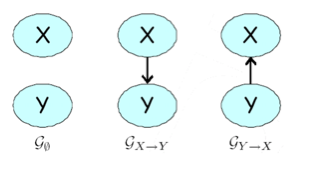
\includegraphics[width=0.4\textwidth]{assets/imap_example.png}
\caption{\label{fig:imap_example}} I-map example
\end{figure}

Example:

Consider a joint probability space over two independent random variables \(X\) and \(Y\) . There are three possible graphs (as shown in Figure \ref{fig:imap_example}) over these two nodes: \(G_\emptyset\), which is a disconnected pair \(X\) \(Y\) ; \(G_{X\rightarrow Y}\) , which has the edge \(X\rightarrow Y\) ; and \(G_{X\rightarrow Y}\) , which contains \(Y\rightarrow X\). The graph \(G_\emptyset\) encodes the assumption that \((X \perp Y )\). The latter two encode no independence assumptions.

Consider following two distributions:

\begin{table}[!htbp]
\parbox{.3\linewidth}{
\begin{tabular}{cc|c}
\(X\) & \(Y\) & \(P(X, Y)\)\\ \hline
\(x^0\) & \(y^0\) & \(0.08\)\\
\(x^0\) & \(y^1\) & \(0.32\)\\
\(x^1\) & \(y^0\) & \(0.12\)\\
\(x^1\) & \(y^1\) & \(0.48\)\\
\end{tabular}
\hfill\hfill
\parbox{.3\linewidth}{
\begin{tabular}{cc|c}
\(X\) & \(Y\) & \(P(X, Y)\)\\ \hline
\(x^0\) & \(y^0\) & \(0.4\)\\
\(x^0\) & \(y^1\) & \(0.3\)\\
\(x^1\) & \(y^0\) & \(0.2\)\\
\(x^1\) & \(y^1\) & \(0.1\)\\
\end{tabular}
}
}
\end{table}

In the example on the left, \(X\) and \(Y\) are independent in \(P\); for example, \(P(x^1) = 0.48 + 0.12 = 0.6\), \(P(y^1) = 0.8\), and \(P(x^1, y^1) = 0.48 = 0.6 · 0.8\). Thus, \((X \perp Y ) \in I(P)\), and we have that \(G_\emptyset\) is an I-map of \(P\). In fact, all three graphs are I-maps of \(P\): \(I(G_{X\rightarrow Y})\) is empty, so that trivially \(P\) satisfies all the independences in it (similarly for \(G_{Y\rightarrow X}\) ). In the example on the right, \((X \perp Y) \not\in I(P)\), so that \(G_\emptyset\) is not an I-map of \(P\). Both other graphs are I-maps of \(P\).

\subsection{Local independences}

\begin{Defn}
A Bayesian network structure \(G\) is a directed acyclic graph whose nodes represent random variables \(X_1,\ldots,X_n\) . Let \(Pa_{X_i}\) denote the parents of \(X_i\) in \(G\), and \(NonDescendants_{X_i}\) denote the variables in the graph that are not descendants of \( X_i\) . Then \(G\) encodes the following set of \textbf{local conditional independence assumptions} \(I_l (G)\):
\[For\ each\ variable\ X_i: (X_i \perp NonDescendant_{X_i} | Pa_{x_i}).\]
\end{Defn}

In other words, a node \(X_i\) is independent of any non descendants given its parents.

\section{D-separation}

\textbf{Direct connection}\quad The simple case is that \(X\) and \(Y\) are directly connected via an edge, say \(X \rightarrow Y\). For any network structure \(G\) that contains the edge \(X \rightarrow Y\) , it is possible to construct a distribution where \(X\) and \(Y\) are correlated regardless of any evidence about any of the other variables in the network. In other words, if \(X\) and \(Y\) are directly connected, we can always get examples where they influence each other, regardless of \(Z\).

\begin{figure}[!bth]
\centering
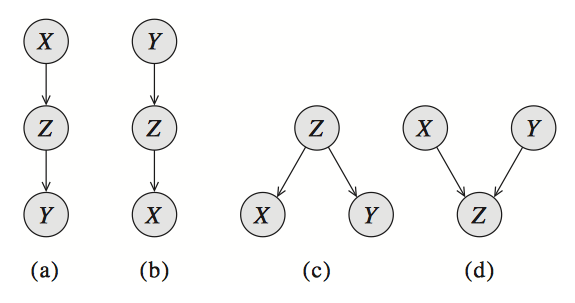
\includegraphics[width=.6\linewidth]{assets/xyz_trail.png}
\caption{\label{fig:xyz_trail} The four possible two-edge trails from \(X\) to \(Y\) via \(Z\)}
\end{figure}

\textbf{Indirect connection}\quad Now consider the more complicated case when X and Y are not directly connected, but there is a trail between them in the graph. We begin by considering the simplest such case: a three-node network, where X and Y are not directly connected, but where there is a trail between them via Z. It is clear that there are four cases where X and Y are connected via Z, as shown in Figure \ref{fig:xyz_trail}.

\begin{itemize}
\item Causal trail \(X \rightarrow Y \rightarrow Z\), and evidential trail \(X \leftarrow Y \leftarrow Z\): active iff \(Z\)is not observed. These two is shown in Figure \ref{fig:xyz_trail} (a),(b)
\item Common cause \(X \leftarrow Z \rightarrow Y\) : active iff \(Z\) is not observed.
\item Common effect \(X \rightarrow Z \leftarrow Y\) : active iff \(Z\) or one of its descendants is observed.
\end{itemize}

\begin{Defn}
Let \(\mathbf{X}\), \(\mathbf{Y}\) , \(\mathbf{Z}\) be three sets of nodes in \(G\). We say that \(\mathbf{X}\) and \(\mathbf{Y}\) are d\textrm{-}separated given \(\mathbf{Z}\), denoted \(d-sep_G(\mathbf{X} ; \mathbf{Y} \ |\ \mathbf{Z})\), if there is no active trail between any node \(X \in \mathbf{X}\) and \(Y \in \mathbf{Y}\) given \(\mathbf{Z}\). We use \(I(G)\) to denote the set of independences that correspond to d-separation:
\[I(G) = \{(\mathbf{X}\perp{\mathbf{Y}}\ |\ \mathbf{Z})\ :\ d\textrm{-}sep_G(\mathbf{X} ; \mathbf{Y} \ |\ \mathbf{Z})\}.\]
This set is also called the set of \textbf{global Markov independences}.
\end{Defn}

\section{Soundness and completeness}

\textbf{Soundness}\quad If a distribution \(P\) factorizes according to a graph \(G\), then \(I(G) \subseteq I(P\)).

\textbf{Completeness}\quad d-separation detects all possible independences.

However, it is important to note that if \(X\) and \(Y\) are not d-separated given \(G\), then it is not the case that \(X\) and \(Y\) are dependent given \(Z\) in all distributions that factorize over \(G\). For example, consider the graph \(A \rightarrow B\). Clearly, \(A\) and \(B\) are dependent. Note that every distribution over \(A\) and \(B\) factorizes according to this graph, since it is always true that \(P(A, B) = P(A)P(B\ |\ A)\). But if we consider the specific distribution give in Table 1, then \(A \perp B\). However, we can assert that if \(X\) and \(Y\) are not d-separated given \(Z\), then there is at least one distribution which factorizes according to the graph, and where \(X\) is not independent of \(Y\) given \(Z\). Combining this with the above theorems gives us an important result.

\begin{table}[!hbt]
\centering
\begin{tabular}{c|cc}
 & \(b^0\) & \(b^1\)\\ \hline
\(a^0\) & 0.4 & 0.6\\
\(a^1\) & 0.4 & 0.6\\
\end{tabular}
\caption{\label{table:completeness} The distribution specified in this table factorizes according to the graph \(A \rightarrow B\) but \(A\) is independent of \(B\).}
\end{table}

\section{Uniqueness of BN}
Very different BN graphs can actually be equivalent, in that they encode precisely the same set of conditional independence assertions.For example, the three networks in figure \ref{fig:xyz_trail}(a),(b),(c) encode precisely the same independence assumption: \(X\perp Y\ |\ Z\). Note that the v-structure network in figure \ref{fig:xyz_trail}(d) induces a very different set of d-separation assertions, and hence it does not fall into the same I-equivalence class as the first three.

\begin{Defn}
Two graph structures \(K^1\) and \(K^2\) over X are I-equivalent if \(I(K^1) = I(K^2)\). The set of all graphs over \(X\) is partitioned into a set of mutually exclusive and exhaustive I-equivalence classes, which are the set of equivalence classes induced by the I-equivalence relation.\(\)
\end{Defn}

\begin{Defn}
The skeleton of a Bayesian network graph \(\mathcal{G}\) over \(X\) is an undirected graph over \(X\) that contains an edge \(\{X, Y\}\) for every edge \((X, Y)\) in \(\mathcal{G}\).
\end{Defn}

\begin{thm}
Let \(\mathcal{G}^1\) and \(\mathcal{G}^2\) be two graphs over \(X\). If \(\mathcal{G}^1\) and \(\mathcal{G}^2\) have the same skeleton and the same set of v-structures then they are I-equivalent.
\end{thm}

\section{Minimum I-Map}

Complete graph is a trivial I-map for any distribution over all variables, since it does not reveal any of the independence structure in the distribution.

\begin{Defn}
A graph \(\mathcal{K}\) is a minimal I-map for a set of independences \(\mathcal{I}\) if it is an I-map for \(\mathcal{I}\), and if the removal of even a single edge from \(\mathcal{K}\) renders it not an I-map.
\end{Defn}

\section{Perfect Maps}

\begin{Defn}
We say that a graph \(\mathcal{K}\) is a perfect map (P-map) for a set of independences \(I\) if we have that \(I(\mathcal{K}) = I\). We say that \(\mathcal{K}\) is a perfect map for \(P\) if \(I(\mathcal{K}) = I(P)\).
\end{Defn}

Note that not every distribution has a perfect map.

\section{Summary}
\begin{itemize}
\item \begin{Defn}
\(A\) Bayesian network is a pair \(B = (G, P)\) where \(P\) factorizes over \(G\), and where \(P\) is specified as a set of CPDs associated with \(G’s\) nodes. The distribution \(P\) is often annotated \(P_B\).
\end{Defn}
\item BN utilizes local and global independences to give a compact representation of the joint distribution.
\item Joint likelihood is computed by multiplying CPDs.
\item Local and global independences are identifiable via d-separation.
\end{itemize}

\end{document}


